% !TEX root = ../thesis.tex

\chapter{Anhang}
\label{anhang}

\begin{figure}[H]
    \centering
    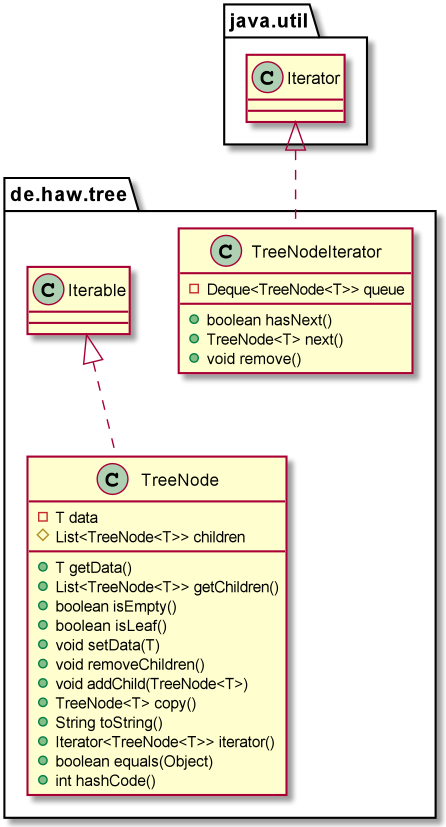
\includegraphics[width=6cm]{../images/tree.png}
    \caption{Baumstruktur}
    \label{tree}
\end{figure}

\begin{figure}[H]
    \centering
    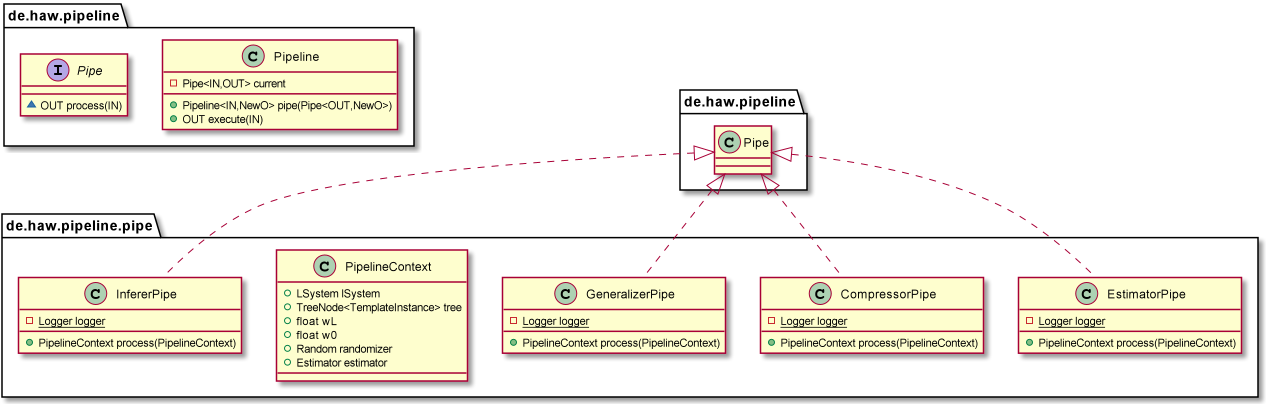
\includegraphics[width=22cm,angle=90]{../images/pipeline.png}
    \caption{Pipeline}
    \label{pipeline}
\end{figure}

\begin{figure}[H]
    \centering
    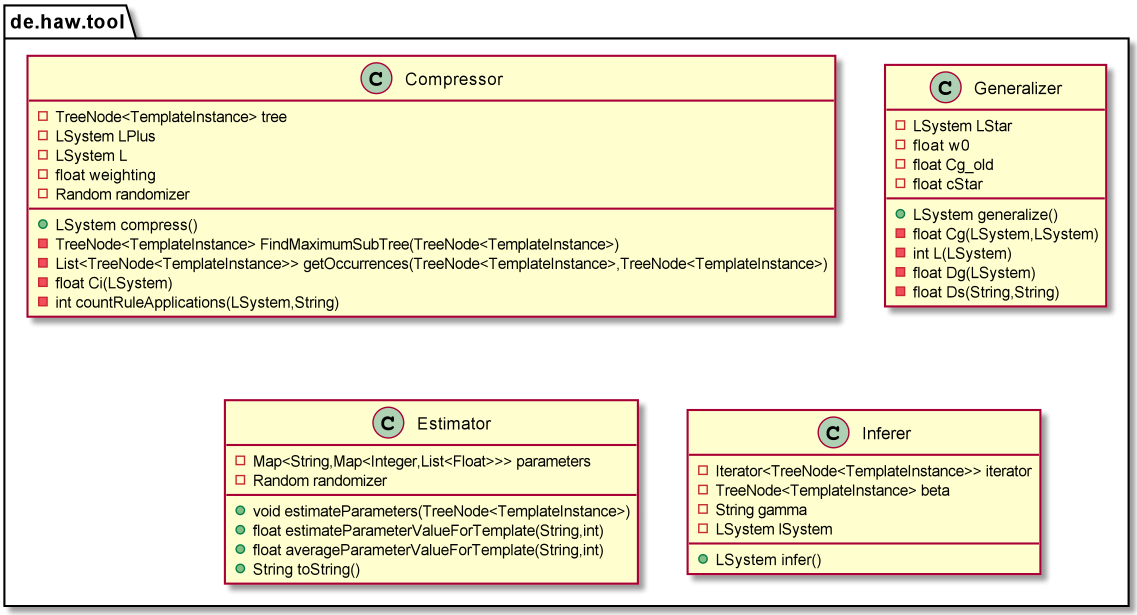
\includegraphics[width=14.8cm]{../images/tool.png}
    \caption{Subsysteme der Generierungs-Pipeline}
    \label{tool}
\end{figure}

\begin{figure}[H]
    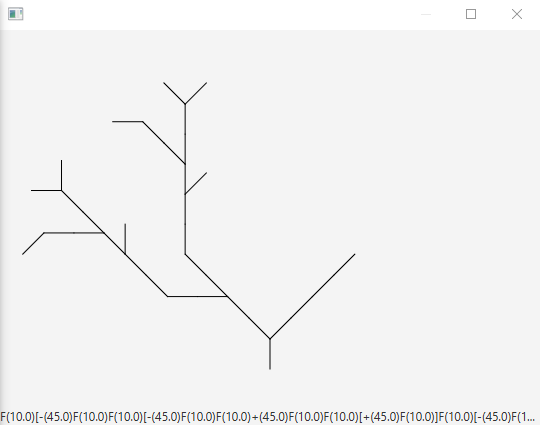
\includegraphics[width=6cm]{../images/example_1.png}
    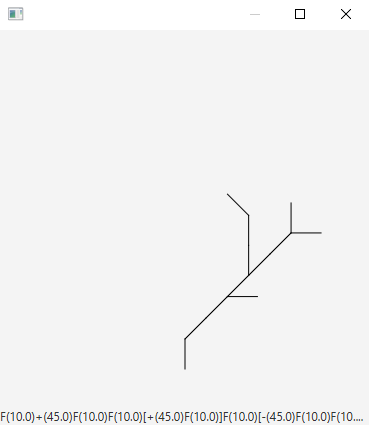
\includegraphics[width=6cm]{../images/example_2.png}
    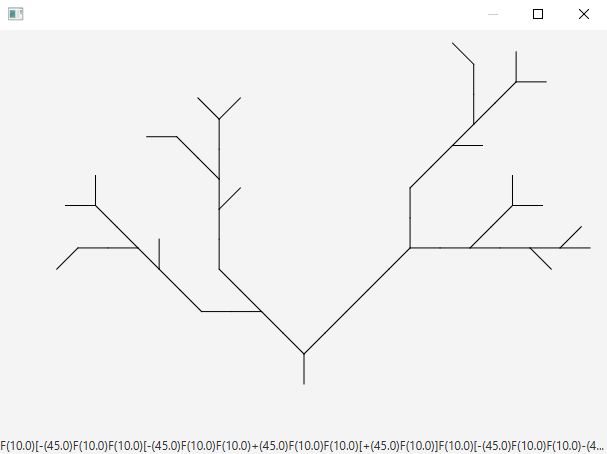
\includegraphics[width=6cm]{../images/example_3.png}
    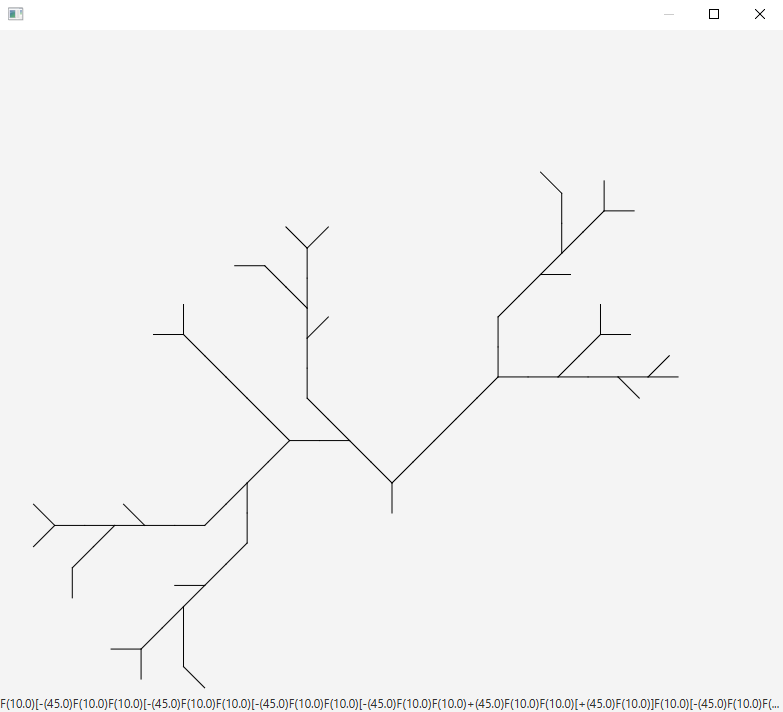
\includegraphics[width=6cm]{../images/example_4.png}
    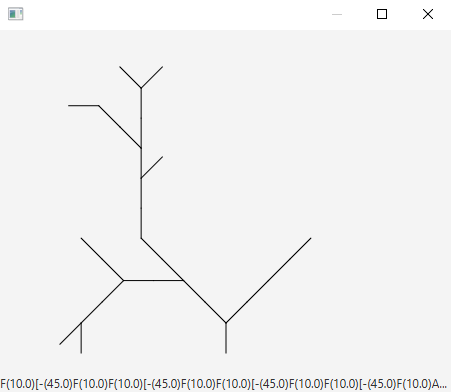
\includegraphics[width=6cm]{../images/example_5.png}
    \caption{Generierte Verzweigungsstrukturen}
    \label{resulting_structures}
\end{figure}

\newpage

\begin{lstlisting}[
    label=treestructure,
    basicstyle=\footnotesize,
    commentstyle=\color{comment},
    keywordstyle=\color{keyword},
    language=Java,
    caption=Klasse TreeNode zur Erstellung einer Baumstruktur,
    frame=tB,
    numberstyle=\color{gray}
]
/**
 * Iterable tree node structure containing a payload and children
 * as tree nodes. Every node represents a whole tree
 */
public class TreeNode<T> implements Iterable<TreeNode<T>> {
    private T data;// Payload
    protected List<TreeNode<T>> children;// Child nodes
    ...
    @Override
    public Iterator<TreeNode<T>> iterator() {
        return new TreeNodeIterator<>(this);
    }
    ...
}
\end{lstlisting}

\begin{lstlisting}[
    label=iterator,
    basicstyle=\footnotesize,
    commentstyle=\color{comment},
    keywordstyle=\color{keyword},
    language=Java,
    caption=Klasse TreeNodeIterator als Iterator für die Baumstruktur,
    frame=tB,
    numberstyle=\color{gray}
]
/**
 * Tree node iterator for iterating nodes of a tree
 * @param <T> Payload of the tree nodes
 */
public class TreeNodeIterator<T> implements Iterator<TreeNode<T>>{
    ...
    @Override
    public boolean hasNext() {
        return !queue.isEmpty();
    }

    @Override
    public TreeNode<T> next() {
        if (queue.isEmpty()) return null;
        var node = queue.pop();
        queue.addAll(node.getChildren());
        return node;
    }
}
\end{lstlisting}

\newpage

\begin{lstlisting}[
    label=pipeline1,
    basicstyle=\footnotesize,
    commentstyle=\color{comment},
    keywordstyle=\color{keyword},
    language=Java,
    caption=Pipeline Klasse zur Organisation von Prozessen,
    frame=tB,
    numberstyle=\color{gray}
]
/**
 * Pipeline class to set up a pipeline design pattern.
 * Classes implementing the Pipe interface can be executed in a specific
 * order while updating a pipeline context
 * @param <IN> Pipeline input type
 * @param <OUT> Pipeline output type
 */
public class Pipeline<IN, OUT> {
    private final Pipe<IN, OUT> current;

    public Pipeline(Pipe<IN, OUT> pipe) {
        current = pipe;
    }

    public <NewO> Pipeline<IN, NewO> pipe(Pipe<OUT, NewO> next) {
        return new Pipeline<>(input -> next.process(current.process(input)));
    }

    public OUT execute(IN input) {
        return current.process(input);
    }
}
\end{lstlisting}

\begin{lstlisting}[
    label=pipeline2,
    basicstyle=\footnotesize,
    commentstyle=\color{comment},
    keywordstyle=\color{keyword},
    language=Java,
    caption=Pipe Interface als Vorlage zur Erstellung eines Teilprozesses einer Pipeline,
    frame=tB,
    numberstyle=\color{gray}
]
/**
 * Pipe class as a process to be part of a pipeline
 * @param <IN> Pipe input type
 * @param <OUT> Pipe output type
 */
public interface Pipe<IN, OUT> {
    OUT process(IN input);
}
\end{lstlisting}

\newpage

\begin{lstlisting}[
    label=ctx,
    basicstyle=\footnotesize,
    commentstyle=\color{comment},
    keywordstyle=\color{keyword},
    language=Java,
    caption=Erstellen des Pipeline Kontextes,
    frame=tB,
    numberstyle=\color{gray}
]
...
var ctx = new PipelineContext();
...
// Execute pipeline
var result = new Pipeline<>(new InfererPipe())
        .pipe(new CompressorPipe())
        .pipe(new GeneralizerPipe())
        .pipe(new EstimatorPipe())
        .execute(ctx);
...
\end{lstlisting}

\begin{lstlisting}[
    label=inferer,
    basicstyle=\footnotesize,
    commentstyle=\color{comment},
    keywordstyle=\color{keyword},
    language=Java,
    numberstyle=\color{gray},
    caption=Inferer Klasse zur Inferierung eines L-Systems aus einer Baumstruktur,
    frame=tB,
    numbers = left
]
/**
 * Inferer to infer a L-System out of a tree-like data structure
 */
public class Inferer {
    ...
    public Inferer(TreeNode<TemplateInstance> tree) {
        //// Initializing
        lSystem = new LSystem();
        // M = {F, S}
        lSystem.addModule("F","S");
        // w = S
        lSystem.setAxiom("S");
        // R <- { alpha: S -> A }
        var alpha = new ProductionRule("S", "A");
        lSystem.addProductionRule(alpha);
        // beta = next node
        beta = iterator.next();
        // M <- gamma in { A, B, ..., Z }, with gamma not in M
        gamma = lSystem.addModuleNotPresentInAlphabet();
    }
    ...
}
\end{lstlisting}

\newpage

\begin{lstlisting}[
    label=infererpipe,
    basicstyle=\footnotesize,
    breaklines = true,
    commentstyle=\color{comment},
    keywordstyle=\color{keyword},
    language=Java,
    numberstyle=\color{gray},
    numbers = left,
    caption=InfererPipe Klasse als Teilprozess der Pipeline,
    frame=tB,
    postbreak=\mbox{\textcolor{gray}{\ArrowBoldDownRight}\space}
]
/**
 * Pipe for executing the infer algorithm.
 * It takes the pipeline context, set it accordingly to the result
 * and returns it to the next pipe
 */
public class InfererPipe implements Pipe<PipelineContext, PipelineContext>, Logging {
    ...
    @Override
    public PipelineContext process(PipelineContext input) {
    ...
    // Update pipeline context
    input.lSystem = new Inferer(input.tree).infer();
    ...
    }
}
\end{lstlisting}

\begin{lstlisting}[
    label=infer,
    basicstyle=\footnotesize,
    breaklines = true,
    commentstyle=\color{comment},
    keywordstyle=\color{keyword},
    language=Java,
    numberstyle=\color{gray},
    numbers = left,
    caption=Inferierungsalgorithmus der Inferer Klasse,
    frame=tB,
    postbreak=\mbox{\textcolor{gray}{\ArrowBoldDownRight}\space}
]
/**
 * Return a L-System inferred from the given tree structure
 * @return Inferred L-System
 */
public LSystem infer() {
    var done = false;
    while (!done) {
        // delta = word of beta
        var delta = (beta == null || beta.isEmpty()) ? "" : beta.getData().getTemplate().getWord();
        // For all variables in delta
        var variableMatches = Pattern.compile("[A-EG-Z]")
                .matcher(delta)
                .results()
                .collect(Collectors.toList());
        for (var v : variableMatches) {
            var index = delta.indexOf(v.group(0));
            // Add new module not present in the alphabet
            String zeta = lSystem.addModuleNotPresentInAlphabet();
            // Replace variable with new module not present in alphabet
            delta = delta.substring(0, index) + zeta + delta.substring(index + 1);
        }

        // R <- { gamma -> delta }
        lSystem.addProductionRule(new ProductionRule(gamma, delta));

        // Find an eta that is in the alphabet but not part of the LHS of any production rule
        var modules = lSystem.getAlphabet();
        for (var eta : modules) {
            if (eta.equals("F")) continue;
            if (eta.equals("S")) continue;
            var lhs = lSystem.getProductionRules().stream()
                    .map(ProductionRule::getLhs)
                    .filter(x -> x.equals(eta))
                    .findFirst()
                    .orElse(null);

            if (lhs == null) {
                gamma = eta;
                break;
            }

            // There is no symbol in the alphabet not being part of a lhs of a production rule?
            if (modules.indexOf(eta) == modules.size() - 1) done = true;
        }
        beta = iterator.next();
    }
    return lSystem;
}
\end{lstlisting}

\newpage

\begin{lstlisting}[
    label=komp,
    basicstyle=\footnotesize,
    breaklines = true,
    commentstyle=\color{comment},
    keywordstyle=\color{keyword},
    language=Java,
    numberstyle=\color{gray},
    numbers = left,
    caption=Klasse Compressor zur Komprimierung eines L-Systems,
    frame=tB,
    postbreak=\mbox{\textcolor{gray}{\ArrowBoldDownRight}\space}
]
/**
 * Compressor class for compressing a L-System.
 * The algorithms searches for identical, maximal subtrees
 * and replaces them with combined instances
 */
public class Compressor {
    ...
    public Compressor(TreeNode<TemplateInstance> tree, LSystem lSystem, float wL, Random randomizer) {
        //// Initializing
        this.tree = tree.copy();
        this.LPlus = lSystem;
        // L = {}
        this.L = new LSystem();
        // wl in [0, 1]
        weighting = wL;
        this.randomizer = randomizer;
    }
    ...
}
\end{lstlisting}

\begin{lstlisting}[
    label=compress,
    basicstyle=\footnotesize,
    breaklines = true,
    commentstyle=\color{comment},
    keywordstyle=\color{keyword},
    language=Java,
    numberstyle=\color{gray},
    numbers = left,
    caption=Komprimierungsalgorithmus der Compressor Klasse,
    frame=tB,
    postbreak=\mbox{\textcolor{gray}{\ArrowBoldDownRight}\space}
]
/**
 * Return a compressed L-System by finding maximum sub-trees
 * and replacing them
 * @return Compressed L-System
 */
public LSystem compress() {
    // T' <- T
    var subtree = FindMaximumSubTree(tree);
    while (subtree != null && !subtree.isEmpty()) {
        // Get extended string representation from (repetitive) sub tree
        var subTreeDerivation = new Inferer(subtree).infer().derive();
        // Data to be set in the tree to replace old node structure representing the subtree
        Template template = new Template(subTreeDerivation);
        // Estimate parameters for new template instance derivation
        var estimator = new Estimator(randomizer);
        var occurrences = getOccurrences(subtree, tree);
        // Average parameter
        for (var o : occurrences) {
            estimator.estimateParameters(o);
        }
        // Replace occurrences of the sub tree
        for (var o : occurrences) {
            var derivationInstance = new TemplateInstance(template);

            int scalingSum = 0, rotationSum = 0, branchingAngleSum = 0;
            int counter = 0;
            for (var node : o) {
                if (node.isEmpty()) continue;
                counter++;
                scalingSum += estimator.averageParameterValueForTemplate("Scaling", node.getData().getTemplate().getId());
                rotationSum += estimator.averageParameterValueForTemplate("Rotation", node.getData().getTemplate().getId());
                branchingAngleSum += estimator.averageParameterValueForTemplate("Branching angle", node.getData().getTemplate().getId());
            }

            derivationInstance.setParameter("Scaling", (float) (scalingSum / counter));
            derivationInstance.setParameter("Rotation", (float) (rotationSum / counter));
            derivationInstance.setParameter("Branching angle", (float) (branchingAngleSum / counter));

            o.setData(derivationInstance);
            o.removeChildren();
        }
        L = new Inferer(tree).infer().minimize();
        if (Ci(L) >= Ci(LPlus)) {
            break;
        }
        // T <- T'
        subtree = FindMaximumSubTree(tree);
        // L+ <- L
        LPlus = L;
    }

    return LPlus.clean();
}
\end{lstlisting}

\newpage

\begin{lstlisting}[
    basicstyle=\footnotesize,
    breaklines = true,
    commentstyle=\color{comment},
    keywordstyle=\color{keyword},
    language=Java,
    linewidth=15cm,
    numberstyle=\color{gray},
    numbers = left,
    caption=Algorithmus zum Finden eines maximalen Unterbaums,
    frame=tB,
    postbreak=\mbox{\textcolor{gray}{\ArrowBoldDownRight}\space}
]
/**
 * Search and for maximum sub-tree that appears more than one time
 * in the tree and return it
 * @param tree Tree to be searched
 * @return Maximum sub-tree
 */
private TreeNode<TemplateInstance> FindMaximumSubTree(TreeNode<TemplateInstance> tree) {
    var globalIterator = tree.iterator();
    globalIterator.next();
    // Iterate
    while (globalIterator.hasNext()) {
        var globalNode = globalIterator.next();
        var localIterator = tree.iterator();
        var l = localIterator.next();
        while (l != globalNode) l = localIterator.next();
        while (localIterator.hasNext()) {
            var localNode = localIterator.next();
            if (!globalNode.isLeaf()) {
                // Check for equality / check for appearance > 1 in the tree
                if (Trees.compare(globalNode, localNode)) return globalNode;
            }
        }
    }
    return null;
}
\end{lstlisting}

\newpage

\begin{lstlisting}[
    basicstyle=\footnotesize,
    breaklines = true,
    commentstyle=\color{comment},
    keywordstyle=\color{keyword},
    language=Java,
    numberstyle=\color{gray},
    numbers = left,
    caption=Algorithmus zum Finden aller Vorkommen eines Unterbaums,
    frame=tB,
    postbreak=\mbox{\textcolor{gray}{\ArrowBoldDownRight}\space}
]
/**
 * Find all occurrences of a sub-tree in a tree
 * @param subtree Sub-tree to be searched for
 * @param tree Tree that contains the sub-tree
 * @return List of sub-trees
 */
private List<TreeNode<TemplateInstance>> getOccurrences(TreeNode<TemplateInstance> subtree, TreeNode<TemplateInstance> tree) {
    var iterator = tree.iterator();
    iterator.next();
    // Store occurrences
    var occurrences = new ArrayList<TreeNode<TemplateInstance>>();
    // Iterate through the tree
    while (iterator.hasNext()) {
        var node = iterator.next();
        if (Trees.compare(node, subtree)) {
            // Subtree to be replaced found
            occurrences.add(node);
        }
    }
    return occurrences;
}
\end{lstlisting}

\begin{lstlisting}[
    basicstyle=\footnotesize,
    breaklines = true,
    commentstyle=\color{comment},
    keywordstyle=\color{keyword},
    language=Java,
    numberstyle=\color{gray},
    numbers = left,
    caption=Funktion zur Berechnung der Kosten eines L-Systems,
    frame=tB,
    postbreak=\mbox{\textcolor{gray}{\ArrowBoldDownRight}\space}
]
/**
 * Return the costs of a L-System combining the length of the alphabet
 * and the number of rule applications of the production rules
 * @param lSystem L-System to be measured
 * @return Costs of the L-System
 */
private float Ci(LSystem lSystem) {
    var costs = 0;
    for (var rule : lSystem.getProductionRules()) {
        costs += weighting * rule.getRhs().length() + (1 - weighting) * countRuleApplications(lSystem, rule.getLhs());
    }
    return costs;
}
\end{lstlisting}

\newpage

\begin{lstlisting}[
    basicstyle=\footnotesize,
    breaklines = true,
    commentstyle=\color{comment},
    keywordstyle=\color{keyword},
    language=Java,
    numberstyle=\color{gray},
    numbers = left,
    caption=Funktion zur Ermittlung der Anzahl Anwendungen einer Produktionsregel,
    frame=tB,
    postbreak=\mbox{\textcolor{gray}{\ArrowBoldDownRight}\space}
]
/**
 * Counts the production rule applications in a string and returns it
 * @param lSystem L-System to be searched
 * @param lhs LHS of a production rule
 * @return Number of production rule applications
 */
private int countRuleApplications(LSystem lSystem, String lhs) {
    int occurrences = 0;
    var pattern = Pattern.compile(lhs);
    // Check axiom
    var axiomMatcher = pattern.matcher(lSystem.getAxiom());
    while (axiomMatcher.find()) occurrences++;
    // Check production rules
    var ruleMatcher = pattern.matcher(lSystem.getProductionRules().stream()
            .map(ProductionRule::getRhs).collect(Collectors.joining()));
    while (ruleMatcher.find()) occurrences++;
    return occurrences;
}
\end{lstlisting}

\begin{lstlisting}[
    basicstyle=\footnotesize,
    breaklines = true,
    commentstyle=\color{comment},
    keywordstyle=\color{keyword},
    language=Java,
    numberstyle=\color{gray},
    numbers = left,
    caption=Generalizer Klasse zur Generalisierung eines L-Systems,
    frame=tB,
    postbreak=\mbox{\textcolor{gray}{\ArrowBoldDownRight}\space}
]
/**
 * Generalizer class to add non-deterministic rules to an L-System
 */
public class Generalizer {
    ...
    public Generalizer(LSystem lSystem, float w0) {
        //// Initialization
        // Generalized grammar L* = L+ (compact grammar)
        LStar = lSystem.copy();
        // metric weight balancing
        this.w0 = w0;
        // C^old_g = Cg(L∗ + {p∗}, L∗)
        Cg_old = 0;
        // cStar
        cStar = 0;
    }
    ...
}
\end{lstlisting}

\newpage

\begin{lstlisting}[
    label=generalize,
    basicstyle=\footnotesize,
    breaklines = true,
    commentstyle=\color{comment},
    keywordstyle=\color{keyword},
    language=Java,
    numberstyle=\color{gray},
    numbers = left,
    caption=Generalisierungsalgorithmus der Generalizer Klasse,
    frame=tB,
    postbreak=\mbox{\textcolor{gray}{\ArrowBoldDownRight}\space}
]
/**
 * Generalize a L-System by adding non-deterministic rules
 * @return Generalized L-System
 */
public LSystem generalize() {
    do {
        // Exclude S -> A from set combinations
        var productionRulesWithoutS = new ArrayList<>(LStar.getProductionRules());
        if (productionRulesWithoutS.remove(0) == null)
            throw new RuntimeException("No rule S -> A found");
        // Generate all possible merging rule pairs P ∈ L*
        var combinations = Sets.combinations(new HashSet<>(productionRulesWithoutS), 2);
        var minimalCosts = Float.MAX_VALUE;
        LSystem minimalLSystem = null;
        // Find a pair p_i with the minimal Cg(L* + {p_i}, L*)
        for (var c : combinations) {
            var LStarMerged = LStar.merge(c);
            float costs = Cg(LStarMerged, LStar);
            if (costs < minimalCosts) {
                minimalCosts = costs;
                minimalLSystem = LStarMerged;
            }
        }
        if (minimalCosts >= 0) break;
        cStar = minimalCosts - Cg_old;
        Cg_old = minimalCosts;
        LStar = minimalLSystem;
    } while (cStar <= 0);

    return LStar;
}
\end{lstlisting}

\newpage

\begin{lstlisting}[
    basicstyle=\footnotesize,
    breaklines = true,
    commentstyle=\color{comment},
    keywordstyle=\color{keyword},
    language=Java,
    numberstyle=\color{gray},
    numbers = left,
    caption=Kostenfunktion zum Vergleich zweier L-Systeme,
    frame=tB,
    postbreak=\mbox{\textcolor{gray}{\ArrowBoldDownRight}\space}
]
/**
 * Calculates the costs of editing a grammar leveraging the grammar
 * length and the grammar edit distance both weighted with a weight
 * balancing w0 ∈ [0.0, 1.0]
 */
private float Cg(LSystem lStar, LSystem lPlus) {
    return w0 * (L(lStar) - L(lPlus)) + (1 - w0) * Dg(lStar);
}
\end{lstlisting}

\begin{lstlisting}[
    basicstyle=\footnotesize,
    breaklines = true,
    commentstyle=\color{comment},
    keywordstyle=\color{keyword},
    language=Java,
    numberstyle=\color{gray},
    numbers = left,
    caption=Längenfunktion über ein L-System,
    frame=tB,
    postbreak=\mbox{\textcolor{gray}{\ArrowBoldDownRight}\space}
]
/**
 * Measure and return the length of a L-System
 * @param lSystem L-System to be measured
 * @return L-System length
 */
private int L(LSystem lSystem) {
    // Set size of the alphabet M
    var M_size = lSystem.getAlphabet().size();
    // Sum of RHS symbols over all production rules
    var sum_rulesRHSs = lSystem.getProductionRules().stream()
            .map(r -> r.getRhs().length())
            .mapToInt(Integer::intValue)
            .sum();
    return M_size + sum_rulesRHSs;
}
\end{lstlisting}

\begin{lstlisting}[
    basicstyle=\footnotesize,
    breaklines = true,
    commentstyle=\color{comment},
    keywordstyle=\color{keyword},
    language=Java,
    linewidth=15cm,
    numberstyle=\color{gray},
    numbers = left,
    caption=Grammar Edit Distance,
    frame=tB,
    postbreak=\mbox{\textcolor{gray}{\ArrowBoldDownRight}\space}
]
/**
 * Grammar edit distance: Overall costs to convert a grammar to another
 * by a set of merging operations M(L+ -> L*)
 */
private float Dg(LSystem lStar) {
    // Grammar edit distance
    var editDistance = 0;
    // Get all multi-module production rules
    var rules = lStar.getProductionRules().stream()
            .filter(rule -> rule.getLhs().length() > 1)
            .collect(Collectors.toList());

    // Go through all merging operations (merging two rules)
    while (!rules.isEmpty()) {
        var operation1 = rules.get(0);
        // Find corresponding rules
        var otherOperations = rules.stream()
                .filter(r -> !r.equals(operation1) && r.getLhs().equals(operation1.getLhs()))
                .collect(Collectors.toList());

        rules.remove(operation1);

        if (!otherOperations.isEmpty()) {
            var iterator = otherOperations.iterator();
            do {
                // Ds(M*_A,M*_B)
                var operation = iterator.next();
                editDistance += Ds(operation1.getRhs(), operation.getRhs());
                rules.remove(operation);
            } while (iterator.hasNext());
        }
    }

    return editDistance;
}
\end{lstlisting}

\begin{lstlisting}[
    basicstyle=\footnotesize,
    breaklines = true,
    commentstyle=\color{comment},
    keywordstyle=\color{keyword},
    language=Java,
    numberstyle=\color{gray},
    numbers = left,
    caption=String Edit Distance,
    frame=tB,
    postbreak=\mbox{\textcolor{gray}{\ArrowBoldDownRight}\space}
]
/**
 * Calculate and return the edit distance between two strings
 * @param M_A String A
 * @param M_B String B
 * @return Edit distance between A and B
 */
private float Ds(String M_A, String M_B) {
    return Modules.editDistanceOptimized(M_A, M_B);
}
\end{lstlisting}

\newpage

\begin{lstlisting}[
    label=editdistance,
    basicstyle=\footnotesize,
    breaklines = true,
    commentstyle=\color{comment},
    keywordstyle=\color{keyword},
    language=Java,
    numberstyle=\color{gray},
    numbers = left,
    caption=Modules Klasse mit Funktion zur Ermittlung der String Edit Distance,
    frame=tB,
    postbreak=\mbox{\textcolor{gray}{\ArrowBoldDownRight}\space}
]
public class Modules {
    ...
    /**
     * Calculate and return the edit distance between two strings
     * @param str1 String A
     * @param str2 String B
     * @return Edit distance between A and B
     */
    public static int editDistanceOptimized(String str1, String str2) {
        int len1 = str1.length();
        int len2 = str2.length();
        int[][] DP = new int[2][len1 + 1];
        for (int i = 0; i <= len1; i++) DP[0][i] = i;
        for (int i = 1; i <= len2; i++) {
            for (int j = 0; j <= len1; j++) {
                if (j == 0) DP[i % 2][j] = i;
                else if (str1.charAt(j - 1) == str2.charAt(i - 1)) DP[i % 2][j] = DP[(i - 1) % 2][j - 1];
                else DP[i % 2][j] = 1 + Math.min(DP[(i - 1) % 2][j], Math.min(DP[i % 2][j - 1], DP[(i - 1) % 2][j - 1]));
            }
        }
        return DP[len2 % 2][len1];
    }
}
\end{lstlisting}

\begin{lstlisting}[
    basicstyle=\footnotesize,
    breaklines = true,
    commentstyle=\color{comment},
    keywordstyle=\color{keyword},
    language=Java,
    numberstyle=\color{gray},
    numbers = left,
    caption=Estimator Klasse zur Erstellung einer Verteilung über Transformaitonsparameter,
    frame=tB,
    postbreak=\mbox{\textcolor{gray}{\ArrowBoldDownRight}\space}
]
/**
 * Estimator class to create a distribution of different
 * transformation parameters
 */
public class Estimator {
    ...
    public Estimator(Random randomizer) {
        /// Initialization
        parameters = new HashMap<>();
        this.randomizer = randomizer;
    }
    ...
}
\end{lstlisting}

\begin{lstlisting}[
    label=estimate,
    basicstyle=\footnotesize,
    breaklines = true,
    commentstyle=\color{comment},
    keywordstyle=\color{keyword},
    language=Java,
    numberstyle=\color{gray},
    numbers = left,
    caption=Verteilungsalgorithmus der Estimator Klasse,
    frame=tB,
    postbreak=\mbox{\textcolor{gray}{\ArrowBoldDownRight}\space}
]
...
/**
 * Create transformation parameter distribution of a given tree
 * @param tree Tree the parameters are distributed from
 */
public void estimateParameters(TreeNode<TemplateInstance> tree) {
    // Determine different parameters
    tree.getData().getParameters().forEach((key, value) -> parameters.putIfAbsent(key, new HashMap<>()));
    // Iterate tree and extract parameters
    for (var node : tree) {
        if (node == null || node.isEmpty()) continue;
        var templateID = node.getData().getTemplate().getId();
        for (var p : node.getData().getParameters().entrySet()) {
            var parameterEntry = parameters.get(p.getKey());
            var templateEntry = parameterEntry.get(templateID);
            if (templateEntry == null) {
                var valueList = new ArrayList<Float>();
                valueList.add(p.getValue().floatValue());
                parameterEntry.put(templateID, valueList);
            } else {
                templateEntry.add(p.getValue().floatValue());
            }
        }
    }
}
...
\end{lstlisting}

\begin{lstlisting}[
    basicstyle=\footnotesize,
    breaklines = true,
    commentstyle=\color{comment},
    keywordstyle=\color{keyword},
    language=Java,
    numberstyle=\color{gray},
    numbers = left,
    caption=Abrufen eines zufälligen Parameters aus der Verteilung für ein Template,
    frame=tB,
    postbreak=\mbox{\textcolor{gray}{\ArrowBoldDownRight}\space}
]
...
/**
 * Estimate and return a parameter for a given template by name
 * @param parameter Parameter name
 * @param templateID Corresponding template
 * @return Estimated parameter value
 */
public float estimateParameterValueForTemplate(String parameter, int templateID) {
    var entries = parameters.get(parameter).get(templateID);
    return entries.get(randomizer.nextInt(entries.size()));
}
...
\end{lstlisting}

\begin{lstlisting}[
    label=durchschnittparameter,
    basicstyle=\footnotesize,
    breaklines = true,
    commentstyle=\color{comment},
    caption=test algo,
    frame=tB,
    keywordstyle=\color{keyword},
    language=Java,
    linewidth=15cm,
    numberstyle=\color{gray},
    numbers = left,
    caption=Berechnung des Durchschnitts eines Parameters für ein Template,
    frame=tB,
    postbreak=\mbox{\textcolor{gray}{\ArrowBoldDownRight}\space}
]
...
/**
 * Calculate and return the average value for a parameter for a
 * given template by name
 * @param parameter Parameter name
 * @param templateID Corresponding template
 * @return Averaged parameter value
 */
public float averageParameterValueForTemplate(String parameter, int templateID) {
    var entries = parameters.get(parameter).get(templateID);
    return (float) entries.stream().mapToDouble(v -> v).average().orElse(0);
}
...
\end{lstlisting}

\begin{figure}[H]
    \centering
    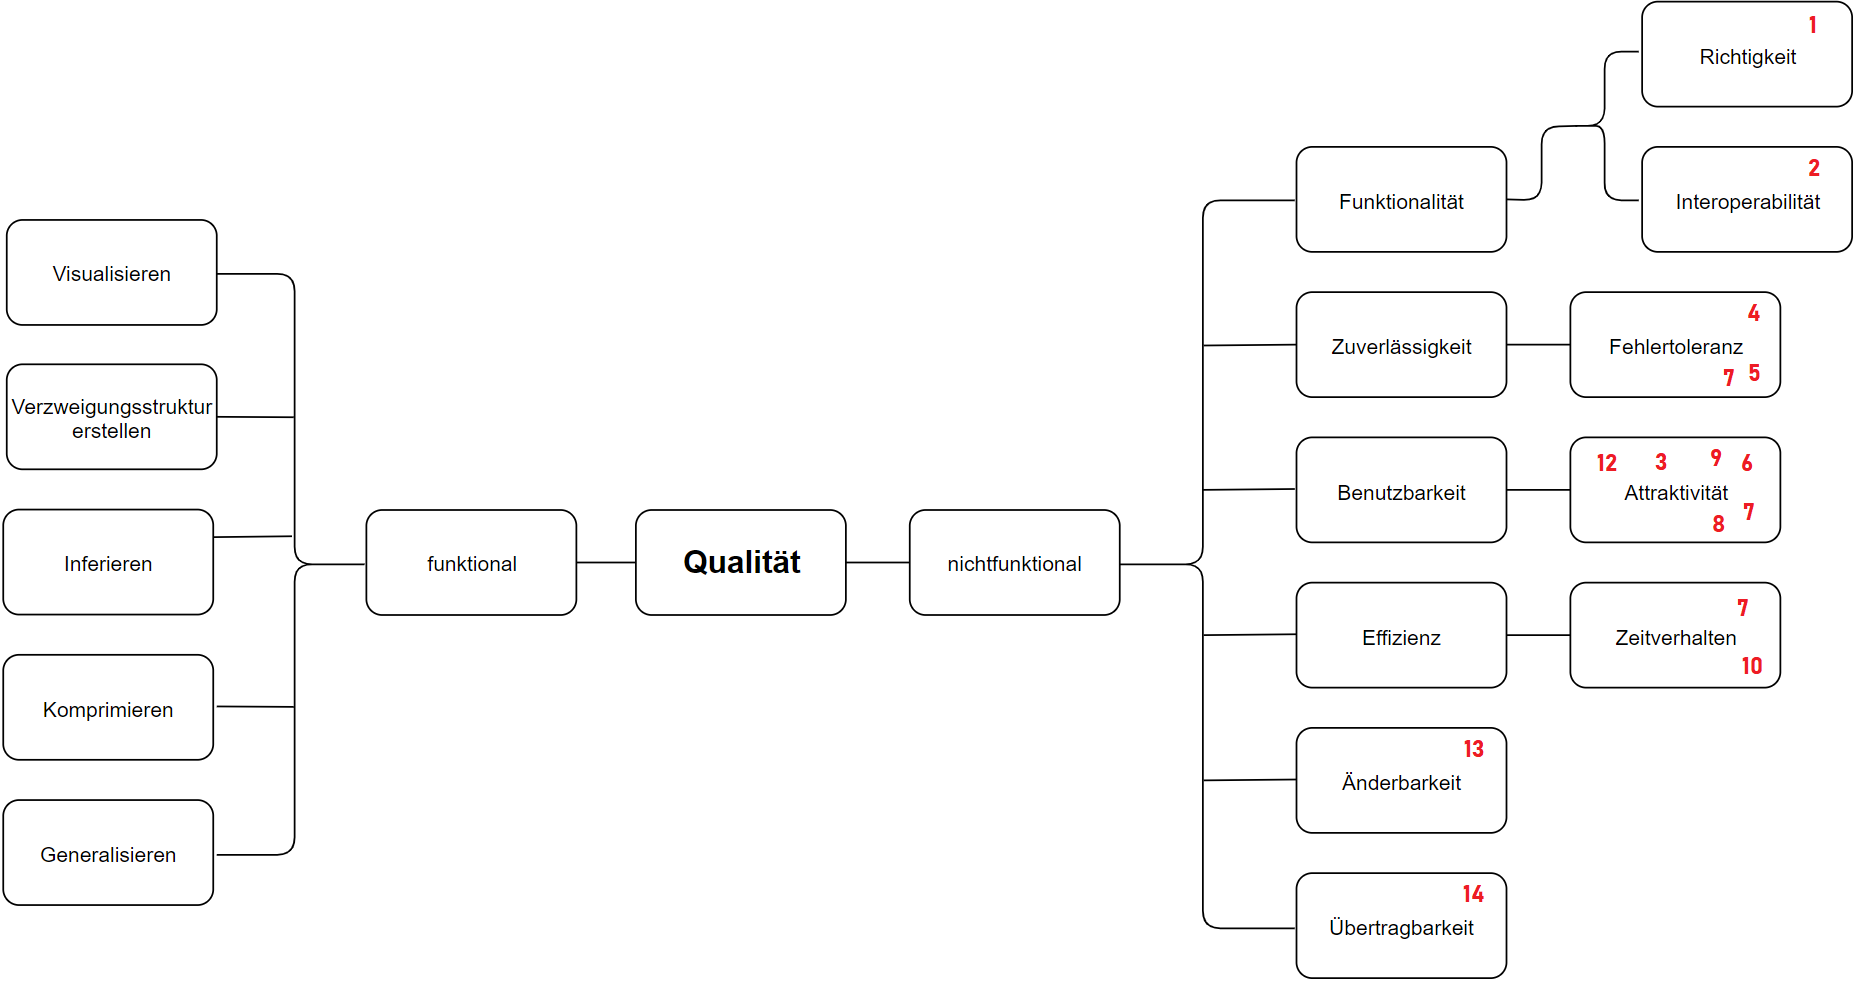
\includegraphics[width=18cm,angle=90]{../images/baum_nummern.png}
    \caption{Qualitätsbaum}
    \label{baum}
\end{figure}